\section{User Roles}\label{sec:fa_roles}

Roles play a very important part in any application: by attaching them to users, they allow the application to authenticate and authorize users based on their roles. If an application has a strong tendency to evolve, so do its roles and authorization sets. This section describes the work involved in making the current system of roles used in \emph{escolinhas.pt} as adaptable as possible.

\subsection{Variability Requirements}\label{sec:fa_roles_variability_requirements}

Authorization is one of the most sensitive areas of any closed software system: it ensures everyone does only what it should in order to guarantee everything works as expected. In a constantly evolving system, the accesses granted by user roles have a tendency to shift and evolve alongside the application --- either because of new features or a new type of user is required in the system to perform specific tasks. In the context of \emph{escolinhas.pt} this problem ties itself with the ACL used: because of the diversity of roles (Fig.~\ref{fig:user_roles_current}) and the three different usage plans, a lot of different rules are applied to determine if a user can or can not perform certain actions; allied to the growing number of features of the platform, this means that the authorization scheme has to be as flexible as possible to ensure minimal overhead when determining new types of permission sets.

\begin{figure}[h]
  \centering
  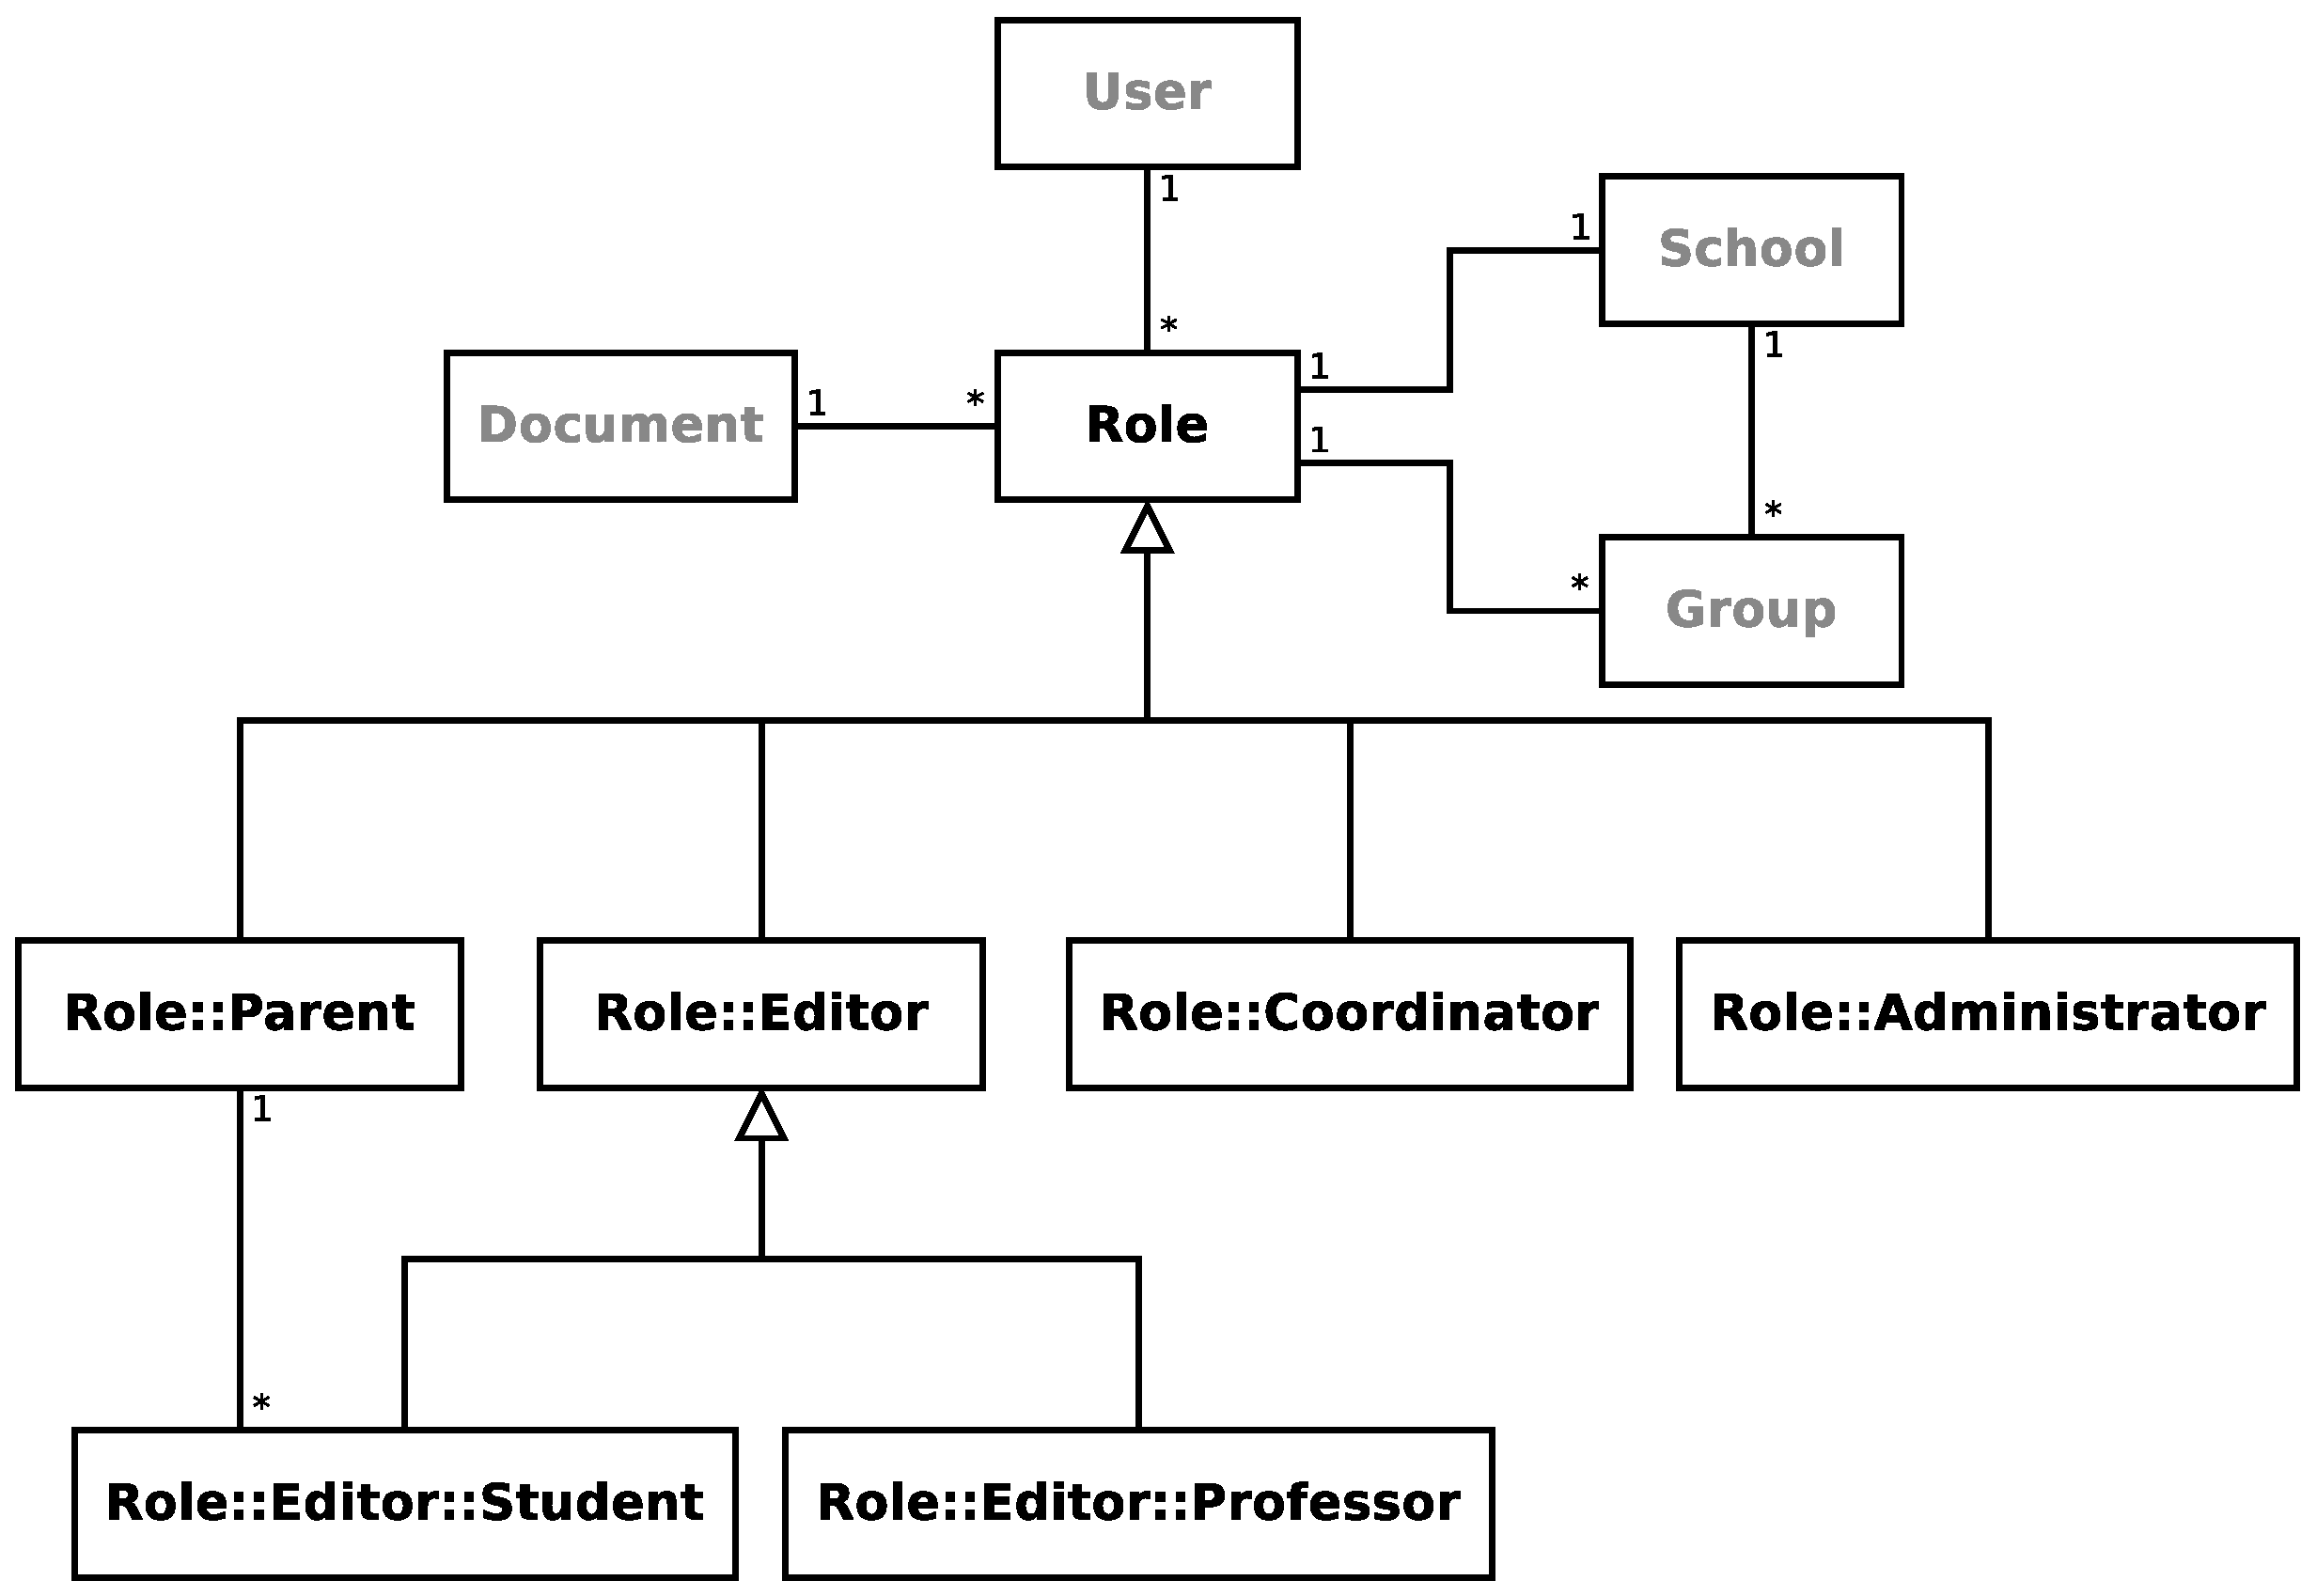
\includegraphics[width=130mm]{user_roles_current}
  \caption{Current User Roles Model.}
  \label{fig:user_roles_current}
\end{figure}

\subsection{Candidate Patterns}\label{sec:fa_roles_candidate_patterns}

The current logic on roles and users states that a user may be a professor, a student, a parent, a coordinator (in which case it also has a professor role associated), or an administrator. Of these five different types of roles, only two of them are allowed editing privileges, which means that only students and professors have to ability to create and edit documents, which leads to an unnecessary level of complexity. If, for example, it was necessary to have a parent with editing privileges, a new Role, descendant of Role::Editor, would have to be created just for that user.

An obvious solution to this problem would be to tie a ``traditional'' \textsc{Access Control List} (as described in~\cite{acls}) to the roles actually in use: this would allow to fine-tune each one of the users permissions and authorization sets while maintaining the codebase clean --- however, the logic surrounding authorization schemas and user roles is built around the \emph{CanCan} Ruby gem~\cite{cancan}, which authorizes an user based on his or her roles, while keeping the necessary logic to a minimum.

As such, the usage of a full-fledged ACL is unnecessary. As \emph{CanCan} rules are written in Ruby and are based on the AR engine used by Rails, \emph{CanCan} is capable of handling authorizations based either on Models (MVC) or \emph{instances} of these Models. The application of an ACL to define user permissions would allow a fine-grained control over the actions of every individual --- instances of \emph{User} Model --- on the system. However, the cases when this kind of control is necessary are rare, which would mean that the increase in complexity brought with the usage of an ACL would not be surpassed by its usefulness: it would be necessary to rewrite every rule already defined within \emph{CanCan} and then associate each user on the system with a specific set of rules, instead of maintaining the current setup and writing a few (rare) exceptions for the users the system administrator saw fit.

\subsection{Chosen Patterns \& Rationale}\label{sec:fa_roles_chosen_patterns_rationale}

As the implementation of an ACL was discarded in \ref{sec:fa_roles_candidate_patterns}, the best solution is to enhance the already present roles system: a flat Role hierarchy, as described in~\cite{baumer_riehle_role_object} would allow for a more flexible authorization scheme, where a User could have one or more roles associated, depending on what actions he would be allowed to do, as shown on Fig.~\ref{fig:user_roles_conceptual}. This also makes the task of creating new roles with different authorization schemes much easier, as there is not a need to conform to any special hierarchy scheme: a new role simply means a new type of user. This clearly contrasts with the previous role's logic, where a multi-level hierarchy was in place.

\begin{figure}[H]
  \centering
  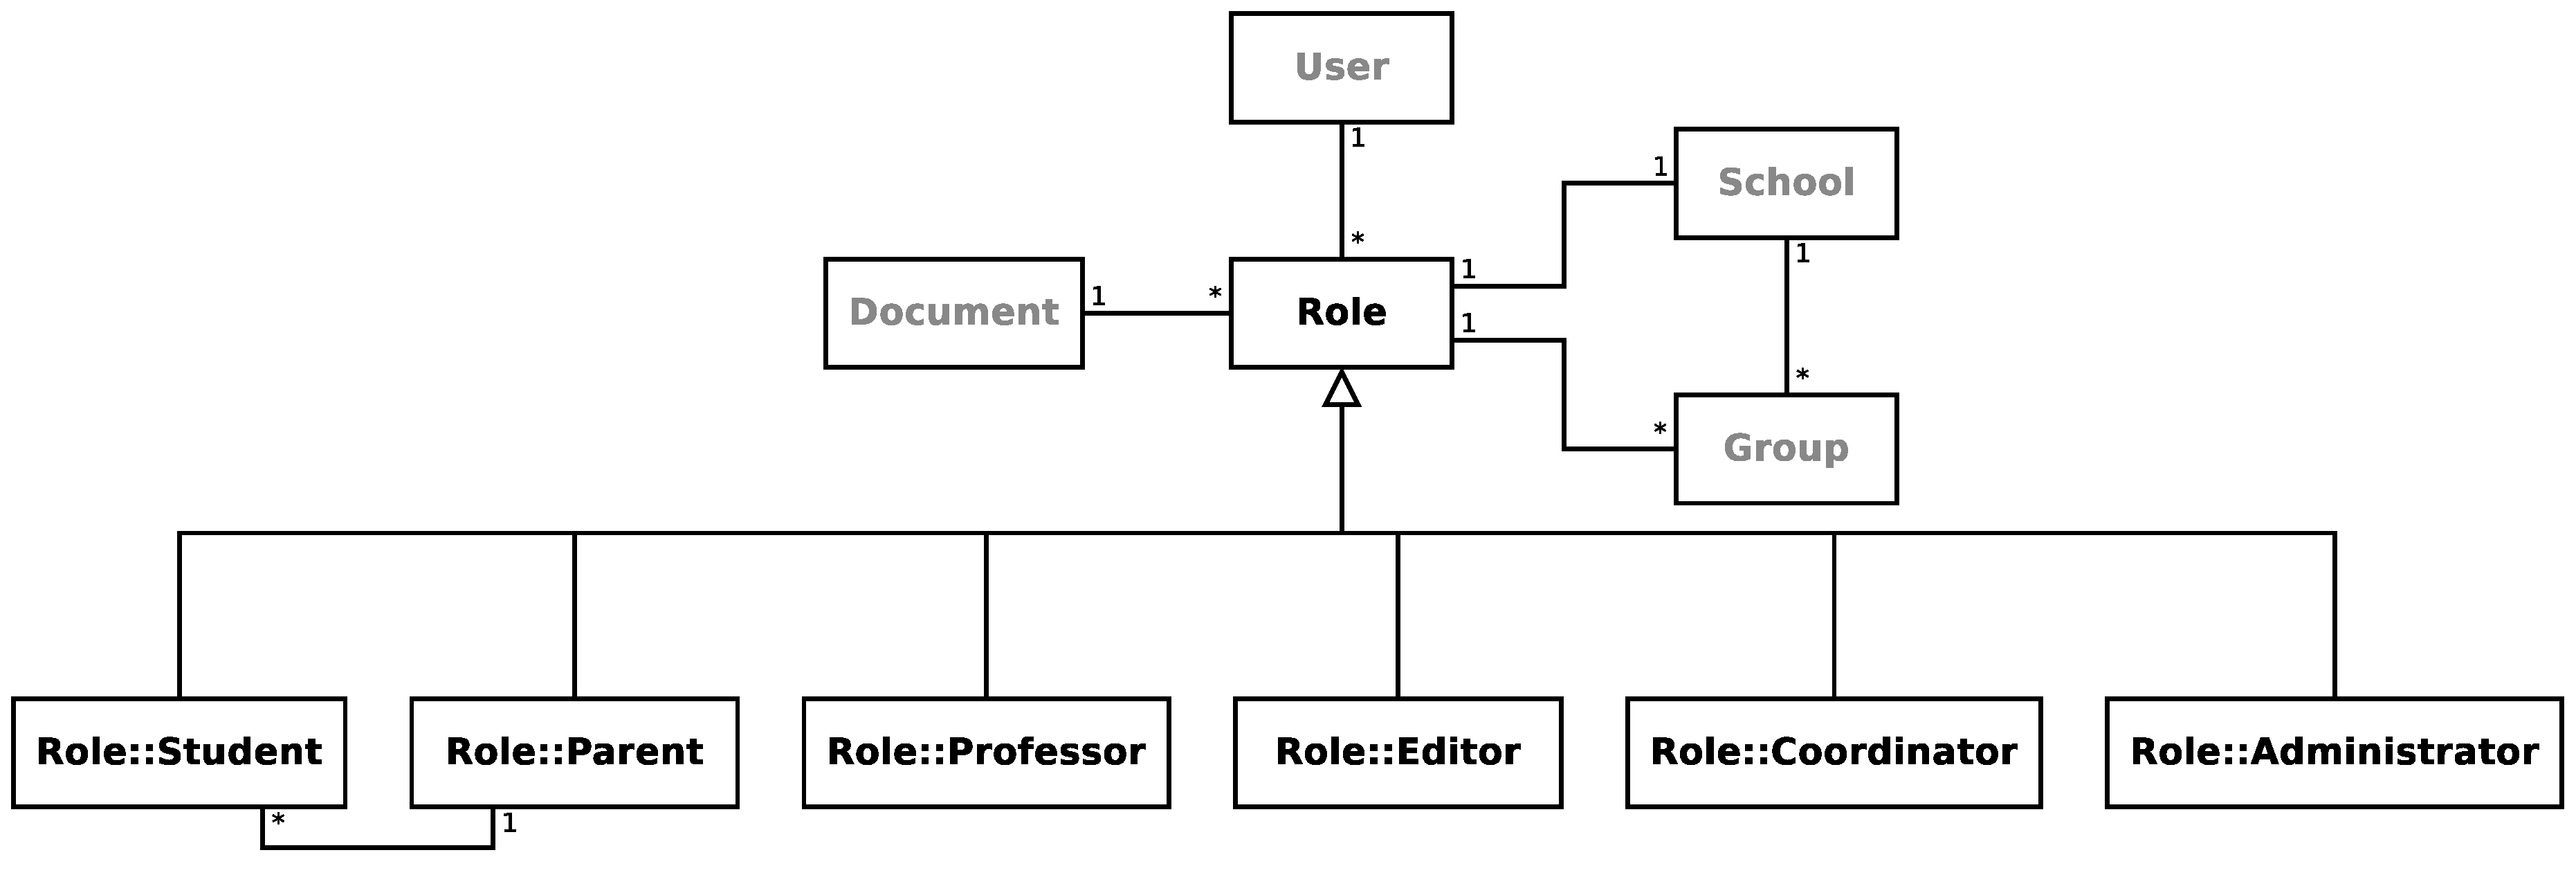
\includegraphics[width=150mm]{user_roles_conceptual}
  \caption{Conceptual User Roles Model.}
  \label{fig:user_roles_conceptual}
\end{figure}

\subsection{Implementation}\label{sec:fa_roles_implementation}

The refactoring of the roles infrastructure was of very low impact, as codebase and database schema are regarded. The hierarchy of Role classes was flattened, keeping it at only two levels: a generic, non-instantiable class \emph{Role}, and all of its currently existent subclasses: \emph{Editor, Parent, Student, Professor, Coordinator} and \emph{Administrator}. Then, the existent rules were adapted to fit this new hierarchy. The last steps pertains to the modification of the current data to fit the new role organization, which entails analyzing each user current roles and performing the adequate substitutions from the previous roles schema. 

\subsection{Impact Analysis}\label{sec:fa_roles_impact_analysis}

The main issues related to the current Roles schema and consequent authorization strategies are caused by the difficulty to capture the constantly evolving necessities of different types of users. As the platform evolves, so do its users and their associated roles. If a new feature is added to the application, it is necessary to define the privileges each user type has over it. The flattening of the Roles hierarchy allows the representation of this Roles as separate, independent objects, allowing the different contexts they refer to be kept separate and also simplify the system configuration.

The usage of a \emph{matricial} ACL implementation, as discussed in \ref{sec:fa_roles_candidate_patterns} would simplify the configuration regarding the privileges of specific users --- allowing a system administrator to have full control over them. Ultimately, this means that the roles would play a very small part in authorization granting, serving only as pre-defined rule sets to be applied to new users.

The usage of a \emph{declarative} ACL (\emph{CanCan}) in conjunction with the \textsc{Role Object} pattern, leads to some important consequences: despite losing the ability to \emph{easily} control the specific set of rules of each user\footnotemark and increasing the difficulty of maintaining constraints between roles, it allows the independent evolution of each \emph{Role}, while making the task of defining their key abstractions regarding each role's position within the platform much more simple and concise.

\footnotetext{This ability  is not completely lost. If necessary, \emph{CanCan} can be used to define authorizations based on a User instance (a specific user)}

%The only relevant point of impact is related to variability. Albeit a low-impact modification, the refactoring of the Roles hierarchy allows for a much quicker role engineering process. This is because a Role now corresponds to a single set of rules, without any hindrance resulting from the previous rule hierarchy. The fact that a multitude of Roles can be associated with a single user allows for a much more wider range of authorizations schemes, as privileges originating from different Roles can be mixed to create unique privilege sets, adapting to a number of different needs.

%\ \\
%\textbf{FIXME: briefly explain how conflicting rules work}




